\documentclass[fleqn]{jbook}
\usepackage{physpub}

\begin{document}

\begin{question}{問題7}{野村}

図1のようなセットアップで、地上において宇宙線を測定する実験を行った。
カウンターBとCとの間には鉛の板が積めるようになっている。

\begin{enumerate}
\item
カウンターA〜Dでは荷電粒子が通過したことを測定する。
荷電粒子の通過を測定する装置としては、一般にどのようなものがあるか。
一つ選んでその原理を簡単に説明せよ。
\end{enumerate}
\parbox{.7\textwidth}{\begin{enumerate}
\setcounter{enumi}{1}
\item
カウンターから出てくる信号を図2の回路によって計数した。
\begin{enumerate}
\item ディスクリミネータは、入力信号があるレベル以上の場合に、
一定の時間幅$\tau$を持つ矩形波を出力する装置である(図3)。
このしきい値のレベルを調整するとき注意すべき点を述べよ。

\item
コインシデンス(同時計数)回路は、2つの入力信号に時間的な重なりが
ある場合に出力パルスを出す。カウンターAからは毎秒$N_\mathrm{A}$
カウント、カウンターBからは毎秒$N_\mathrm{B}$カウントの頻度で、
コインシデンス回路に信号が入るものとする。それぞれの信号の幅を
$\tau$秒とした時、AとBからの独立な信号が偶然重なってコインシデンス
回路から出力が出る頻度はいくらか求めよ。(ただし、AとBの同時計数の
頻度は$N_\mathrm{A}$と$N_\mathrm{B}$に比べてずっと少ないものとする。)
また、図2の可変遅延器はなぜ必要か答えよ。

\item
偶然によるコインシデンス(同時計数)が多すぎると測定が困難になるが、
その場合どのような対策を施したら良いか。

\item 
カウンターや回路には、一度信号が来るとすぐには次の信号を受け付けない
不感時間がある。この測定装置と回路全体の不感時間は$T$秒であった。
スケーラーで測定された計数を毎秒$S$カウントとすると、真の計数はいくつか。

\item
カウンターBとCの間の鉛の板の枚数を変えながらスケーラーのカウント数
を記録すると、図4のようになった。図のx、yに対応する宇宙線粒子は
それぞれ以下にあげる粒子のうちどれか答えよ。また、それらの粒子は
鉛の中でどういう過程でエネルギーを失うのか説明せよ。\[
\hbox{(I)電子、(II)ニュートリノ、(III)ミュー粒子(ミューオン)}
\]

\end{enumerate}
\end{enumerate}}
\parbox{.3\textwidth}{\begin{center}
%$\phantom{x}$\\[6cm]
\input{2000phy7-1.tpc}\\
図1: 測定セットアップ

\end{center}}
\begin{center}
\input{2000phy7-2.tpc}
\end{center}
\begin{enumerate}
\setcounter{enumi}{2}
\item
宇宙線に含まれるミュー粒子を鉛の板で止めてその寿命を測りたい。
ミュー粒子は、およそ2マイクロ秒で電子とニュートリノ2つに崩壊する。
\begin{enumerate}
\item
300MeV/cの運動量を持つミュー粒子を止めるのに必要な鉛の厚さを
図5より求めよ。ここで、$R$は飛程(荷電粒子を止めるのに要する物質量
($\mathrm{g/cm^2}$))、$M$は粒子の質量、$\beta$は粒子速度を光速度で
割ったもの、また$\gamma=\frac{1}{\sqrt{1-\beta^2}}$とする。ただし、
ミュー粒子の質量は$106\mathrm{MeV/c^2}$、鉛の密度は
$11.35\mathrm{g/cm^3}$である。

\item
前問で求めた厚さの鉛の板をカウンターBとCの間に置いた。カウンター
A、B、Cを使ってミュー粒子の寿命を測るにはどのようにしたら良いか。
図2のようなダイアグラムを書いて説明せよ。この測定では実験誤差として
どのようなものが重要か考察せよ。また、カウンターDを使わない理由を書け。

\end{enumerate}\end{enumerate}

\begin{center}
\input{2000phy7-3.tpc}\\
\input{2000phy7-4.tpc}\qquad
%\includegraphics[scale=.5]{2000phy7-1-reduced.eps}図5
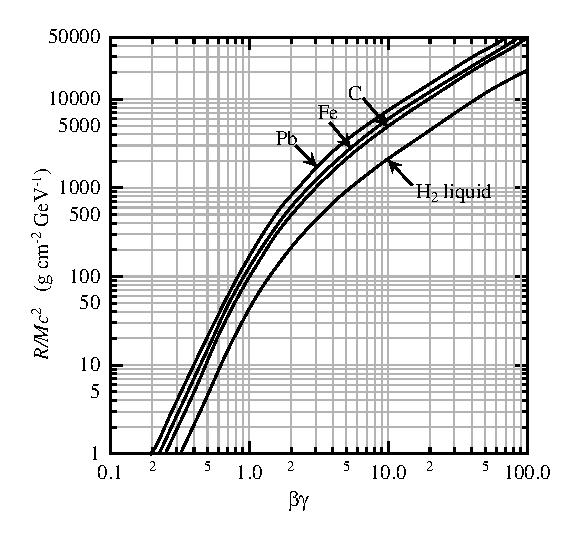
\includegraphics[width=.35\textwidth]{2000physQ7_1.eps}図5
\end{center}
\end{question}
\begin{answer}{問題7}{}
\begin{enumerate}
\item 
荷電粒子の通過を測定する装置の一つとして、シンチレーションカウンターが
ある。シンチレーションカウンターは、シンチレーター(蛍光体)と
光電子増倍管とからできている。

荷電粒子がシンチレーターの中に入射すると、
シンチレーター中の電子と相互作用し、電子を励起させる。
励起した電子は、基底状態にもどるときに光子を放出する。
この光子は光電面に集められ、電子とカップリングして光電子になる。

光電子が光電子増倍管のなかの電極にぶつかると、二次電子が放出される。
この際、電子の数は増幅される。電子は、この衝突・増幅を何回か
くりかえした後、アノード(陽極)に入射して電流をながす。

以上がシンチレーションカウンターの原理である。

解答作成者からの注)ほかに、GM管、比例計数管、霧箱などがありますが、
原理については各自で調べてください。

\item
\begin{enumerate}
\item カウンターから出てくる信号には、環境放射線による
ものが混ざっている。しかし、環境放射線のエネルギーは、宇宙線の
エネルギーにくらべて小さい。つまり、ディスクリミネーターのしきい値を、
環境放射線のエネルギーより大きく、宇宙線のエネルギーより小さいレベルに
設定すれば、宇宙線による信号だけをとりだすことができる。\\

\item
% カウンターAから信号が出力されている時間の割合は、
% $N_\mathrm{A}\tau$である。この時間の間にカウンターBからも
% 出力されるような頻度をもとめればよく、その値は毎秒
% $N_\mathrm{B}\times N_\mathrm{A}\tau$カウントとなる。
%日下君の指摘に従って訂正。
カウンターAの信号の立ち上がりの前後$\pm\tau$の間に
カウンターBの立ち上がりがあれば、コインシデンスが生ずる。
カウンターAの立ち上がり前後$\pm\tau$は、1秒当たり$N_A\cdot 2\tau$あり、
この間にカウンターBが立ち上がるのでさらに$N_B$を掛けて
結局答えは毎秒$2N_AN_B\tau$カウントとなる。


可変遅延線がない場合、宇宙線があるカウンターに入ってから別の
カウンターに入るまでに時間差が生じたり、回路の違いによって
コインシデンス回路に信号がとどくまでに時間差が生じたりする。
可変遅延線は、これらの時間差を調整し、同じ宇宙線による信号が同時に
コインシデンス回路に入るようにするために必要である。

\item 偶然による同時計数が多すぎる場合、カウンターの
数をふやして、すべての信号のコインシデンスをとればよい。$i$番目の
カウンターから信号が出力される時間の割合を$\alpha_i(<1)$とすると、
すべてのカウンターからの信号が重なる確率は、$\prod\alpha_i$となり、
カウンターの数をふやせばふやすほど小さくなることがわかる。

\item
 実際に測定した時間は1秒間あたり$1-TS$秒なので、
真の計数は毎秒$S/(1-TS)$カウントである。

\item  ニュートリノは物質とほとんど相互作用しないため
無視する。

鉛の板を透過しにくい粒子の方が,鉛を厚くしたときのスケーラーの
カウント数の減り方は大きく,そちらがxに対応する.
電子は$\mu$粒子より質量が小さいため,散乱されやすいので,
電子の方が鉛の板を透過しにくいと考えられる.よって,
xが(I)電子,yが(III)$\mu$粒子だと考えることができる.

これらの粒子は、主に電磁相互作用によって電子や原子核に散乱され、
制動輻射で光子を放出してエネルギーを失う。
\end{enumerate}
\item 
\begin{enumerate}
\item  $\mu$粒子が300\,MeVの運動量をもつので、
\begin{eqnarray*}
 \beta\gamma = \frac{p\mathrm{c}}{M\mathrm{c}^2}=2.83
\end{eqnarray*}
となる。すると、問題で与えられた図から
\begin{eqnarray*}
 \frac{R}{M\mathrm{c}^2}
  = 1.5\times10^3\,[\mathrm{g\cdot cm^{-2}\cdot GeV^{-1}}]
\end{eqnarray*}
が得られる。$M\mathrm{c}^2$は0.106\,GeVなので、
\begin{eqnarray*}
 R = 1.5\times10^3\times0.106 = 1.6\times10^2\,[\mathrm{g\cdot cm^{-2}}]
\end{eqnarray*}
となる。鉛の密度は$11.35\,[\mathrm{g/cm^3}]$なので、$\mu$粒子を
止めるのに必要な鉛の厚さは、
\begin{eqnarray*}
 \frac{1.6\times10^3}{11.35} = 14\,[\mathrm{cm}]
\end{eqnarray*}
だとわかる。

\item 図のTACとはTime to Analog Converterのことで、
startが入力されてからstopが入力されるまでの時間をアナログパルスに
変換する回路である。まず、カウンターA、Bを使って、$\mu$粒子が
入射したときにstartに入力する。
$\mu$粒子が鉛の板で止まり、
Cがならなかったことを確認するため、Cの出力をNOTしておく。

しばらくすると$\mu$は崩壊して電子を放出する。
この電子をカウンターBまたは
Cで検出して、stop信号に入力する。こうやって出力されるパルスを
デジタル化して、横軸に時間、縦軸に頻度をとったヒストグラムにすると、
このグラフは$A\exp(-t/\tau)$($\tau$は$\mu$粒子の寿命)という式で
フィットできる。こうして$\mu$粒子の寿命を求めることができる。

可変遅延器の設定であるが、start 信号に関しては、
あまり A, Bからの信号がCよりはやくANDに到達するとCが鳴らなかったのを
確認する以前に start 信号が出てしまうこと、
またあまりはやくBからの信号が OR に到達すると、
start 信号を生成したBの信号がまた stop を生成してしまいお話にならないこと
を注意して設定すべきである。

この実験では、環境放射線や別の$\mu$が
カウンターCに入射してもstop信号が出てしまい、
ヒストグラムに影響を与える。
これらバックグラウンドの大きさが十分小さくないと、
上のフィットは正しくなくなる。
その場合は、$A\exp(-t/\tau)+B$という形でフィットする。
別に環境放射線のみの計数を測っておいて
それからバックグラウンドを推定することもできよう。

カウンターDを使わない理由は,必要ないからである.
$\mu$粒子は鉛の板で止めてしまうので,カウンターDに到達しない.
$\mu$粒子の崩壊の際に生成する電子は,カウンターB,Cで検出するので,
やはりカウンターDは必要ない.
%なお,電子の検出にカウンターA,Dを
%使わない理由は,これらのカウンターが鉛から離れているため,
%放出される電子からみた立体角が小さく,測定されるデータ数が
%減ってしまうためだろう.
\end{enumerate}\end{enumerate}
\begin{center}\input{2000phy7-6.tpc}\end{center}
\end{answer}


\end{document}
